\documentclass{article}
\usepackage[utf8]{inputenc}
\usepackage{graphicx}
\usepackage{subfigure}
\usepackage{float}
\usepackage{indentfirst}
\usepackage{caption}
\usepackage{subcaption}
\usepackage[a4paper,includeheadfoot,margin=3cm]{geometry}
\usepackage{amsmath}
\usepackage[subrefformat=parens,labelformat=parens]{subfig}
%\titleformat{\subsection}{\normalsize}%{}{0em}{}

\title{DD2423 - Image Analysis and Computer Vision\\
  \large Lab 2}
\author{
  Gabriela Zarzar Gandler\\
  \texttt{gzrsm@kth.se}
  \and
 Huijie Wang\\
  \texttt{huijiew@kth.se}
}
\date{November 2016}


\begin{document}

\maketitle


%%%%Extra Questions%%%
% 1. different sign of convolution and filter (if we use a wrong sign, we will end up with opposite direction of curve in edge with smoothing)
% 2. 


\begin{enumerate}
\section{Difference operators}
    \item %Q1
    \textbf{What do you expect the results to look like and why? Compare the size of dxtools with the size of tools. Why are these sizes different?}
    \par
    The result is shown as Figure \ref{fig:q1}:
    \begin{figure}[H]
        \centering
        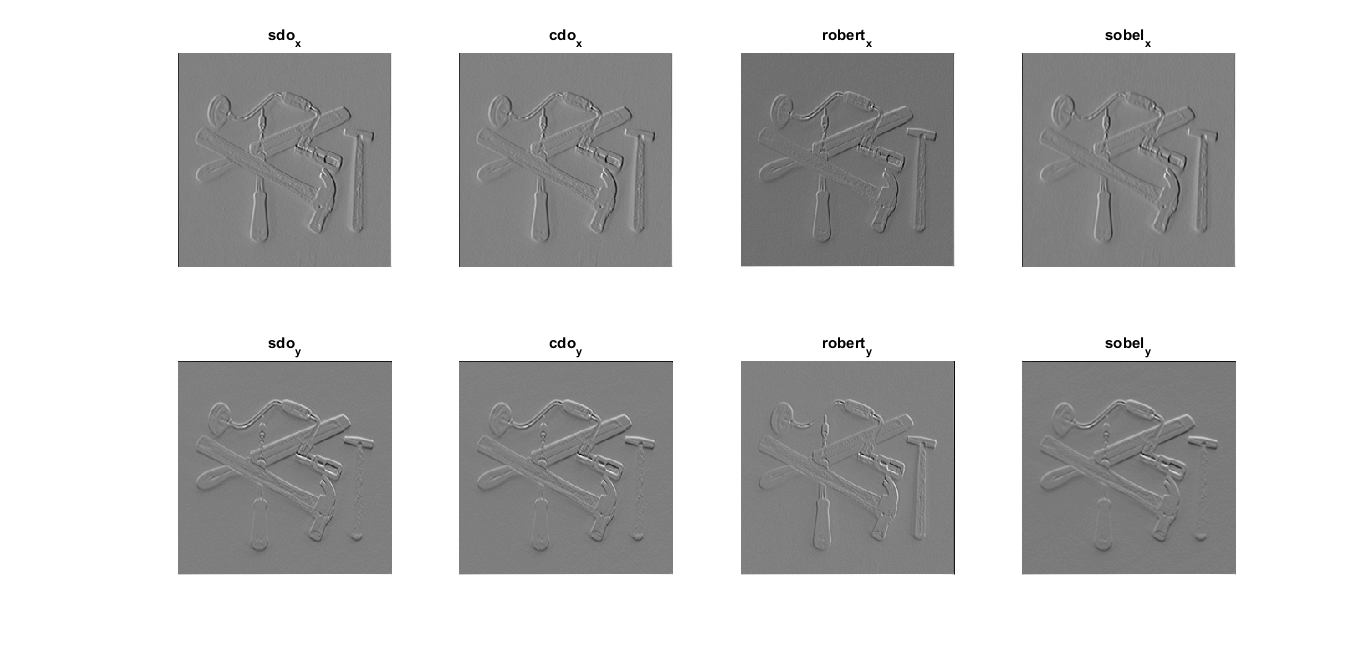
\includegraphics[width=\linewidth]{Lab2-Q1.png}
        \caption{Discrete derivations using difference operators}
        \label{fig:q1}
    \end{figure}
    \par
    We expect the result to highlight places where there are sharp transitions - such as edges - in the x direction and in the y direction. For the Robert operator, particularly, we expect these transitions to be highlighted in the diagonals (45 degrees). These expectations are justified by the filters, which represent derivatives. The size of the image is 256. After applying different filters, the size of \textbf{dxtools} turns out to be $256 \times 254$ for simple and central difference operator, $255 \times 255$ for Robert's diagonal operator and $254 \times 254$ for Sobel opeartor. That is because we use 'valid' as parameter when applying convolution in Matlab, which doesn't add padding to initial image. So that the size after convolution should be $size_x - (size\_filter_x-1) \times  size_y - (size\_filter_y-1)$.
    

    
    % ROBERT OPERATOR
    % The main reason for using the Roberts Cross operator is that it is very quick to compute. Only four input pixels need to be examined to determine the value of each output pixel, and only subtractions and additions are used in the calculation. In addition there are no parameters to set. Its main disadvantages are that since it uses such a small kernel, it is very sensitive to noise. It also produces very weak responses to genuine edges unless they are very sharp. The Sobel operator performs much better in this respect.
    
    % size corresponding to para 'valid' or 'same'

\section{Point–wise thresholding of gradient magnitudes}
    \item %Q2
    \textbf{Is it easy to find a threshold that results in thin edges? Explain why or why not!}
    
    No, it is not easy to find a threshold that results in thin edges, because we are using first-derivatives. This is the problem of solving edge detection by thresholding on the edge strength (gradient magnitude): the resulting edges are often several pixels wide. The first-derivative is usually a ramp-like transition and thresholding may remove too much of certain edges and too little of others.
    %P182!!!!!!!!!!
    \begin{figure}[H]
        \centering
        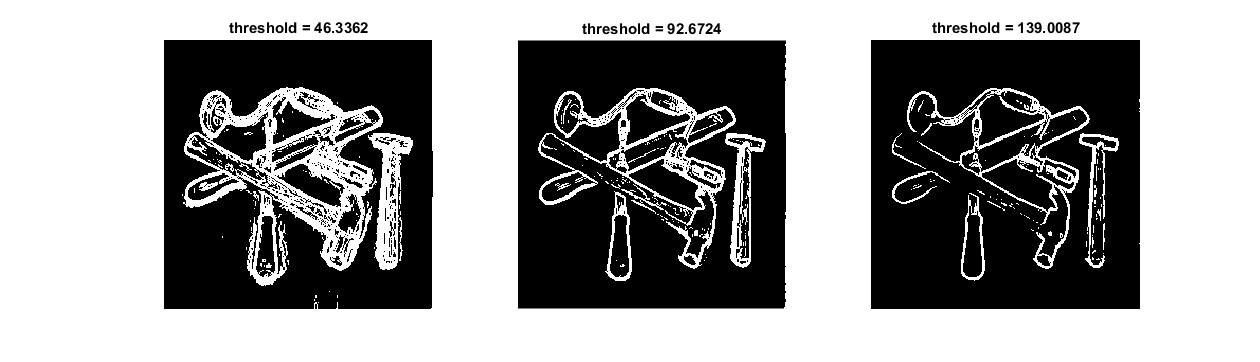
\includegraphics[width=\linewidth]{Lab2-Q2.png}
        \caption{Point–wise thresholding of gradient magnitudes}
        \label{fig:q2}
    \end{figure}
    
    \item %Q3
    \textbf{Does smoothing the image help to find edges?}
    % Kind of.......?
    
    Smoothing reduces the noise, which is very good. The gradient of the original image is much affected by noises. So smoothing the image makes it possible to "trust" more on the sharp transitions that the gradient detects. However there is a trade-off problem: if the image is smoothed too much, the actual edges are not detected, while if the image is not smoothed enough, the edges are still highlighted, but there is also a lot of "false positives" (noise, for example). Smoothing the image also makes the edges thicker, because the intensity "ramps" get longer.
    
    \begin{figure}[H]
        \centering
        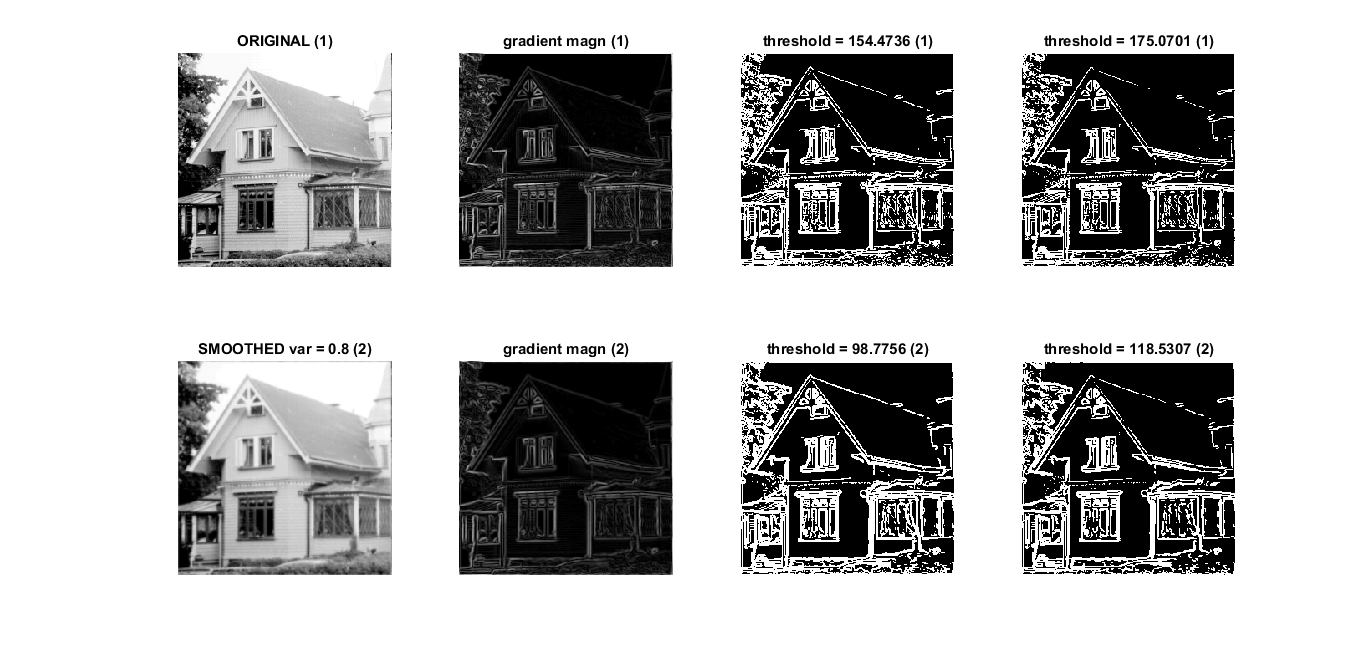
\includegraphics[width=\linewidth]{Lab2-Q3.png}
        \caption{Effect of smoothing}
        \label{fig:q31}
    \end{figure}
    
    \begin{figure}[H]
        \centering
        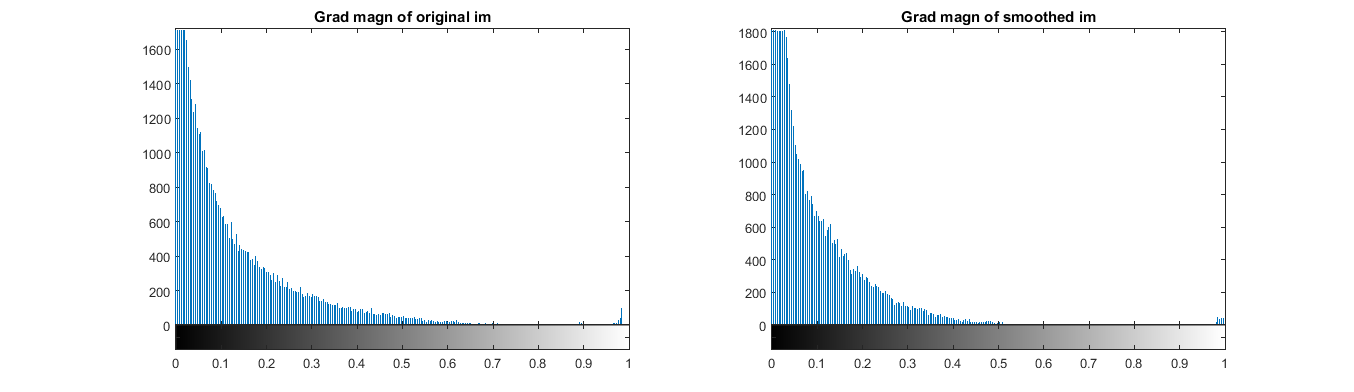
\includegraphics[width=\linewidth]{Lab2-Q3-2.png}
        \caption{Histogram of gradient magnitude before and after smoothing}
        \label{fig:q32}
    \end{figure}
    
    
\section{Differential geometry based edge detection: Theory}

\section{Computing differential geometry descriptors}
    \item %Q4
    \textbf{What can you observe? Provide explanation based on the generated images.}
    
    We can observe in Figure \ref{figq4} that, the larger the scale (variance of the Gaussian filter), the less contour there is. This means that the noises get suppressed - the first image is corrupted by so much contour, due to inconvenient non-smoothed variations in the intensity level. However if one increases the scale too much, there is a loss of valuable information, as the edges get distorted - they tend to get curved, especially on areas close to corners.
    
\begin{figure}[!htb]
\centering
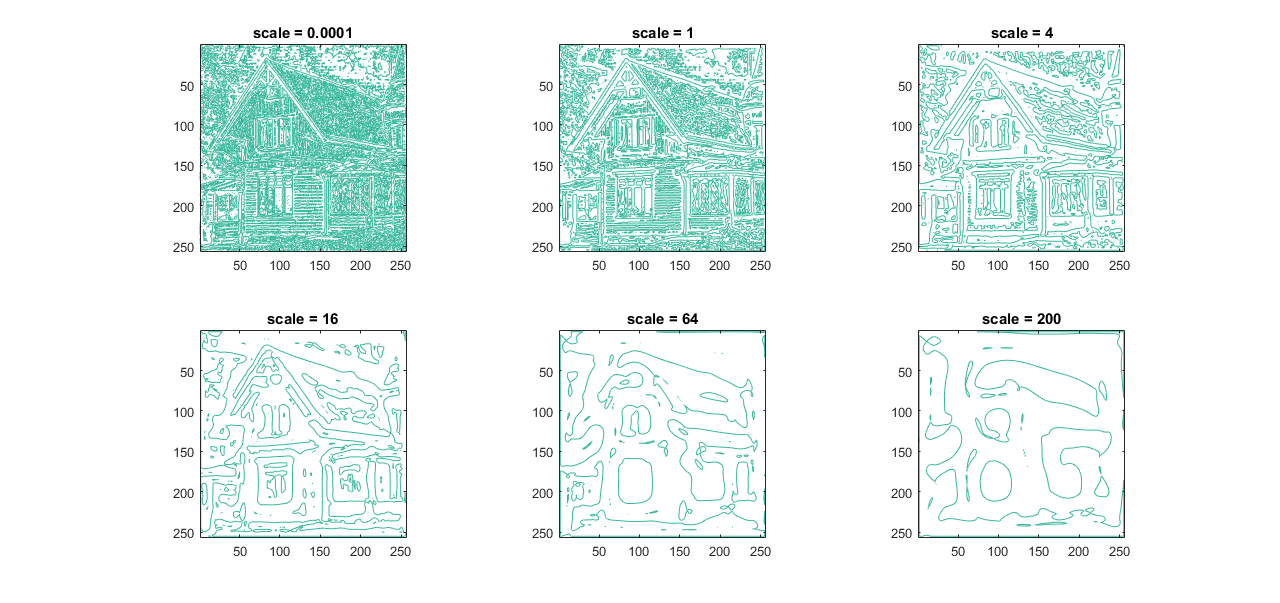
\includegraphics[width=6in]{lab2q4.png}
\caption{Contour of zero-valued second derivative}
\label{figq4}
\end{figure}

    \item %Q5
    \textbf{Assemble the results of the experiment above into an illustrative collage with the subplot command. Which are your observations and conclusions?}

We conclude that the more intense the smoothing is, the less varying the sign of the third derivative is. This makes the areas with negative third derivative thicker. The white areas are followed by a black ``contour'' on the outside, due to the shape of the third derivative in the presence of an edge.

\begin{figure}[!htb]
\centering
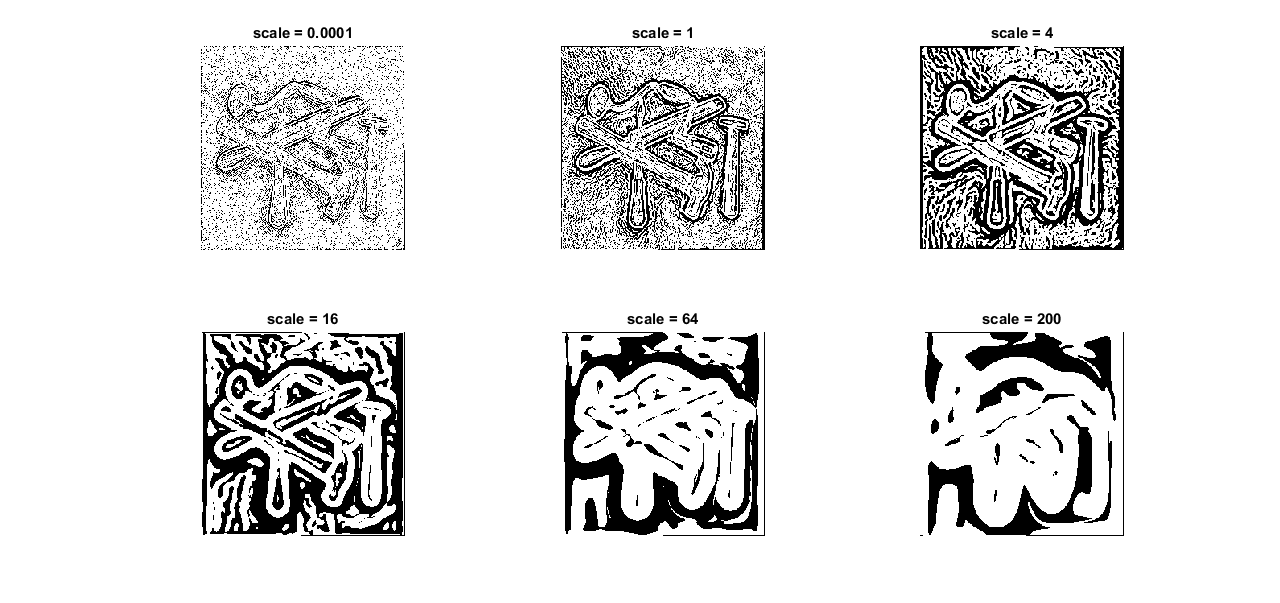
\includegraphics[width=6in]{lab2q5.png}
\caption{Highlighting negative third derivative}
\label{figq5}
\end{figure}

\item %Q6
\textbf{How can you use the response from $\tilde{L}_{vv}$ to detect edges, and how can you
improve the result by using $\tilde{L}_{vvv}$?}

% zero-crossing P725
Firstly we look to the $L_{vv}$ representation of the image. Then we consider only the points of this representation where the third derivative is negative. Finally we plot the contour corresponding to zero-valued pixels. 

    \begin{figure}[H]
        \centering
        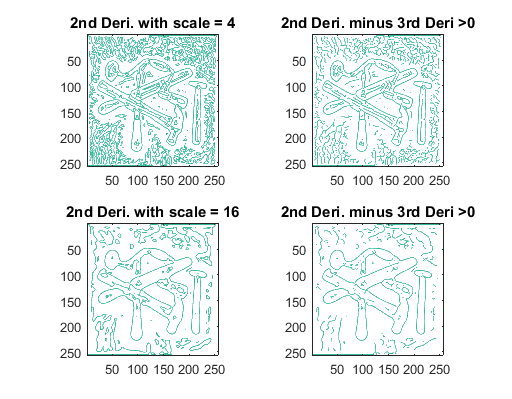
\includegraphics[width=0.7\linewidth]{Lab2-Q6.png}
        \caption{Improving $\tilde{L}_{vv}$ with $\tilde{L}_{vvv}$}
        \label{fig:q6}
    \end{figure}

\section{Extraction of edge segments}

    \item %Q7
    \textbf{Present your best results obtained with extractedge for house and tools.}
    \par
    In Figure \ref{fig:q71}, we can find $scale = 4$ and $threshold = 8$ is a decent value for \textit{Tools} and in Figure \ref{fig:q72}, $scale = 4$ and $threshold = 4$ is a decent value for \textit{House}.
    \par
    Through these images, we can find that a large scale gives curved edges and a too small scale would do poor in eliminating noises.
    %Conclusions: large scale gives curved edges
    
    \begin{figure}[H]
        \centering
        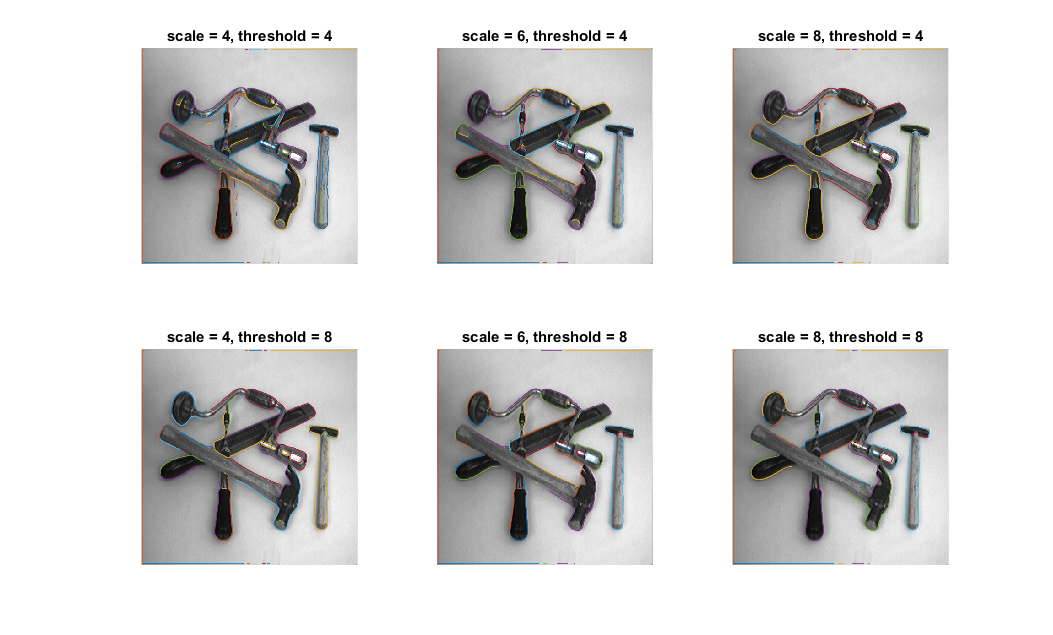
\includegraphics[width=\linewidth]{Lab2-Q7.png}
        \caption{Extraction of edge segments on \textit{Tools}}
        \label{fig:q71}
    \end{figure}
    
    \begin{figure}[H]
        \centering
        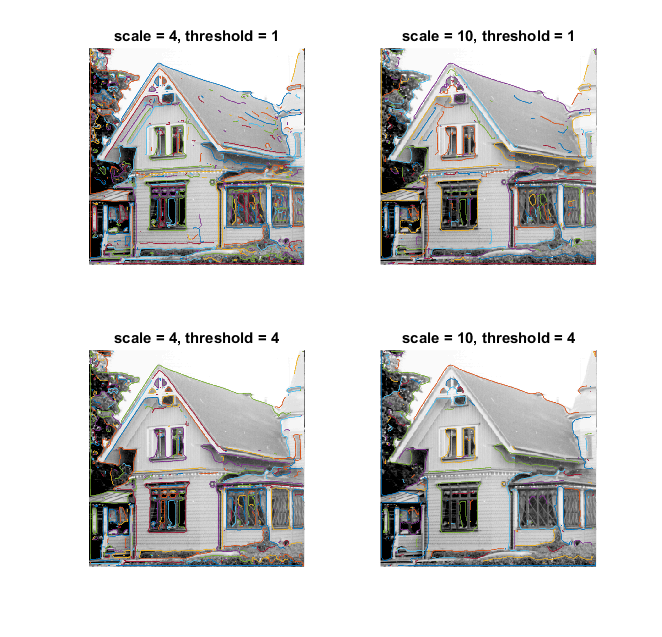
\includegraphics[width=0.7\linewidth]{Lab2-Q7-2.png}
        \caption{Extraction of edge segments on \textit{House}}
        \label{fig:q72}
    \end{figure}

\section{Hough transform}
%P755

\item %Q8
\textbf{Identify the correspondences between the strongest peaks in the accumulator
and line segments in the output image. Doing so convince yourself that the implementation is correct. Summarize the results of this study and print out on paper.}
\par

%Can we observe the reflective adjacency property of Hough transforms?

% Interpret!
The results are shown as Figure \ref{fig:q81} and Figure \ref{fig:q82}. In simple shapes, it is obvious that the detected lines correspond with the maximum points in Hough space.

\item %Q9
\textbf{How do the results and computational time depend on the number of cells
in the accumulator?}
\par
The more cells in the accumulator end up with more computational time. That is because in Hough Transform we use loops to go through every $\theta$ for every edge point.
\par
On the other hand. It is important to find appropriate number of $n \rho$ and $n \theta$. Too large number, especially for $n \rho$, will lead to multiple response to a single line. On the other hand, too small number will lead to low accuracy.

    \begin{figure}[H]
        \centering
        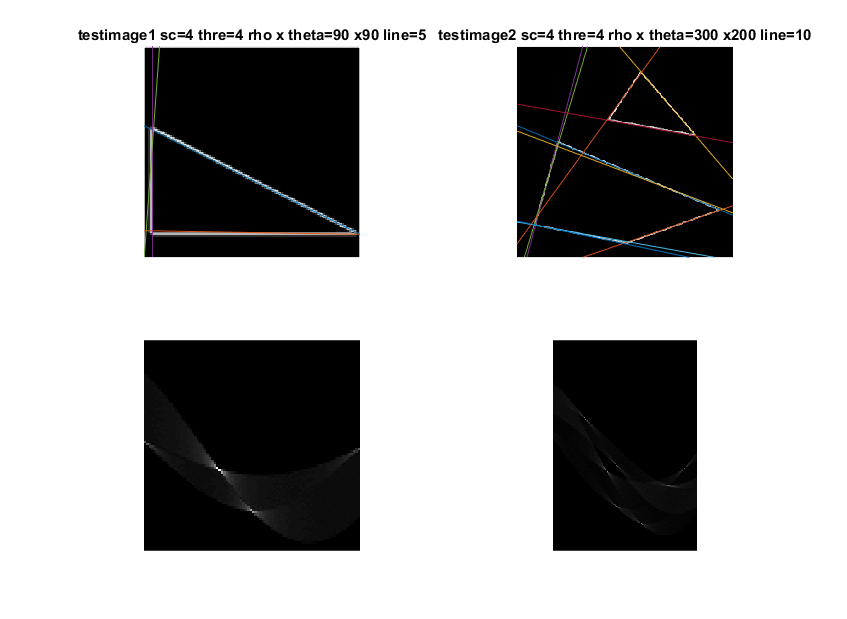
\includegraphics[width=0.6\linewidth]{Lab2-Q8-1.png}
        \caption{Hough transform on simple images}
        \label{fig:q81}
    \end{figure}
    
    \begin{figure}[H]
        \centering
        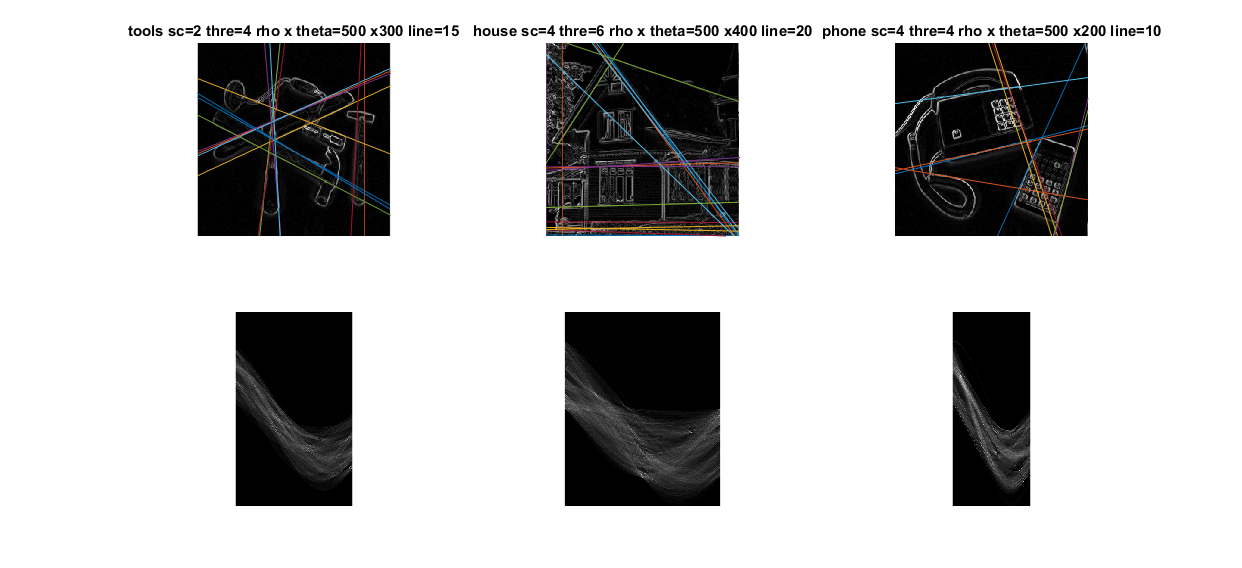
\includegraphics[width=\linewidth]{Lab2-Q8-2.png}
        \caption{Hough transform on complex images}
        \label{fig:q82}
    \end{figure}



\item %Q10
\textbf{How do you propose to do this? Relate your answer to the different parts
of the images.}
\par 
As a larger value of magnitude is more likely to be an edge pixel, using magnitude value or a monotonically increasing function of magnitude can accelerate the increment in Hough space. We tried 4 ways:\\
\quad 1. $increment = 1$.\\
\quad 2. \textit{increment = magnitude of the pixel}.\\
\quad 3. \textit{increment = log(1 + magnitude of the pixel)} .\\
\quad 4. $increment = \sqrt{magnitude \quad of \quad the \quad pixel} $.\\
As a result, seems like the first and third work fine.

\end{enumerate}
\end{document}
